\begin{activity} \label{A:4.1.2}  A ball is tossed vertically in such a way that its velocity function is given by $v(t) = 32 - 32t$, where $t$ is measured in seconds and $v$ in feet per second.  Assume that this function is valid for $0 \le t \le 2$.
\ba
	\item For what values of $t$ is the velocity of the ball positive?  What does this tell you about the motion of the ball on this interval of time values?
	\item Find an antiderivative, $s$, of $v$ that satisfies $s(0) = 0$.  
	\item Compute the value of $s(1) - s(\frac{1}{2})$.  What is the meaning of the value you find?
	\item Using the graph of $y = v(t)$ provided in Figure~\ref{F:4.1.Act2}, find the exact area of the region under the velocity curve between $t = \frac{1}{2}$ and $t = 1$.  What is the meaning of the value you find?
	\item Answer the same questions as in (c) and (d) but instead using the interval $[0,1]$.
	\item What is the value of $s(2) - s(0)$?  What does this result tell you about the flight of the ball?  How is this value connected to the provided graph of $y = v(t)$?  Explain.
\ea
\begin{figure}[h]
\begin{center}
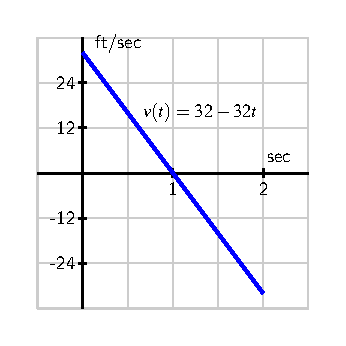
\includegraphics{figures/4_1_Act2.eps}
\end{center}
\caption{The graph of $y = v(t)$.} \label{F:4.1.Act2}
\end{figure}
\end{activity}
\begin{smallhint}
\ba
	\item Where is velocity zero?
	\item Since $v$ is linear, note that $s$ must be quadratic.
	\item Observe that you are taking the difference between two values of the position function.
	\item The region whose area is sought is triangular.
	\item See (c) and (d) above.
	\item What does it mean for the change of the ball's position to be zero?
\ea
\end{smallhint}
\begin{bighint}
\ba
	\item Where is velocity zero? Recall that positive velocity makes the position function increasing.
	\item Since $v$ is linear, note that $s$ must be quadratic.  What function has derivative $32$?  What function has derivative $32t$?
	\item Observe that you are taking the difference between two values of the position function.
	\item The region whose area is sought is triangular.  Simply use the known formula for the area of a triangle; do not use approximating rectangles.
	\item See (c) and (d) above.
	\item What does it mean for the change of the ball's position to be zero?  How should we think of the area that lies beneath the $t$-axis on the interval $1 < t < 2$?
\ea
\end{bighint}
\begin{activitySolution}
\ba
	\item Note that $v(1) = 0$ and for $0 < t < 1$, $v(t) > 0$.  This means that on the interval $(0,1)$, the position function $s$ is increasing because velocity is positive.
	\item We can check that the derivative of $s(t) = 32t - 16t^2$ is $s'(t) = v(t) = 32 - 32t$, and that $s(0) = 0$, so this is the antiderivative of $v$ that we desire.
	\item Now, $s(1) - s(\frac{1}{2}) = (32 - 16) - (16 - 4) = 4$, which is the change in position of the ball on the interval $[\frac{1}{2},1]$.  Equivalently, since $v$ is positive through this interval, 4 feet is the vertical distance the ball traveled during this time.
	\item On the interval from $t = \frac{1}{2}$ to $t = 1$, the corresponding area under the velocity curve is the area of the right triangular region whose width is $\frac{1}{2}$ seconds and whose height is $v(\frac{1}{2}) = 16$ feet/sec.  That area is therefore $A = \frac{1}{2} bh = \frac{1}{2} \cdot \frac{1}{2} \cdot 16 = 4$ feet.  This is the total distance the ball traveled vertically on $[0,\frac{1}{2}]$.
	\item $s(1) - s(0) = (32 - 16) - (0-0) = 16$, which is the vertical distance the ball traveled on the interval $[0,1]$.  The area under the velocity curve on $[0,1]$ is the area of the triangle with height 32 (ft/sec) and base 1 (second), which is $A = \frac{1}{2} \cdot 1 \cdot 32 = 16$ feet.  These two results are identical, in part due to the fact that we are using two different perspectives to compute the same quantity, which is distance traveled.
	\item Observe that $s(2) - s(0) = (32 - 32) - (0 - 0) = 0$.  This means that the ball has zero change in position on the interval $[0,2]$.  But we already established that on the interval $[0,1]$, the ball traveled 16 feet vertically; since the velocity becomes negative on the interval $1 < t < 2$, there we know the ball's position is decreasing, so it is falling back to earth.  The resulting zero change in position means that at $t = 2$ the ball has returned to the location from which it was tossed.  If we view the area between the velocity function and the $t$-axis as being negative wherever $v$ is negative, then we see that the areas of the two triangles involved are opposites, which in some sense results in the ``total area'' being zero, matching the change in position.
\ea
\end{activitySolution}
\aftera